% The s-plane: absolute convergence for Re s > 1, the critical strip, the critical line, the pole at 1, trivial zeros, first non-trivial zeros. Generated by a short script.
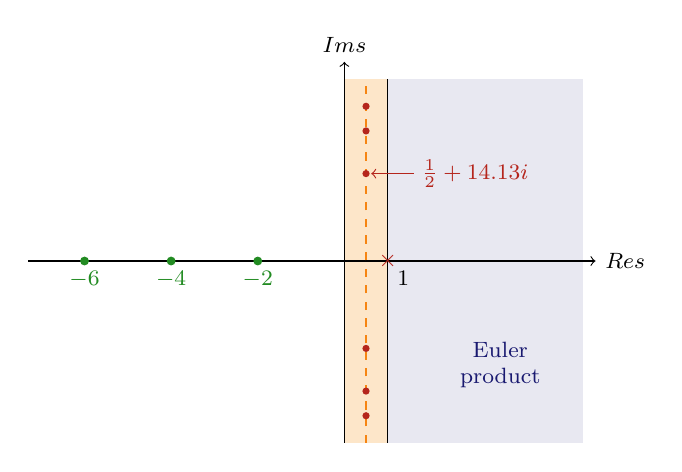
\begin{tikzpicture}[every node/.style={font=\footnotesize}]
\fill[MidnightBlue!10] (0.550,-2.310) rectangle (3.025,2.310);
\fill[BurntOrange!18] (0,-2.310) rectangle (0.550,2.310);
\draw[->] (-4.015,0)--(3.190,0) node[right] {$\operatorname{Re}s$};
\draw[->] (0,-2.310)--(0,2.530) node[above] {$\operatorname{Im}s$};
\draw[BurntOrange,thick,dashed] (0.275,-2.310)--(0.275,2.310);
\draw (0.550,-2.310)--(0.550,2.310);
\node[MidnightBlue,align=center] at (1.980,-1.320) {Euler\\product};
\node[BrickRed] at (0.550,0) {$\times$};\node[below right] at (0.550,0) {$1$};
\fill[ForestGreen] (-1.100,0) circle (1.6pt) node[below] {$-2$};
\fill[ForestGreen] (-2.200,0) circle (1.6pt) node[below] {$-4$};
\fill[ForestGreen] (-3.300,0) circle (1.6pt) node[below] {$-6$};
\fill[BrickRed] (0.275,1.110) circle (1.3pt);
\fill[BrickRed] (0.275,-1.110) circle (1.3pt);
\fill[BrickRed] (0.275,1.652) circle (1.3pt);
\fill[BrickRed] (0.275,-1.652) circle (1.3pt);
\fill[BrickRed] (0.275,1.965) circle (1.3pt);
\fill[BrickRed] (0.275,-1.965) circle (1.3pt);
\draw[BrickRed,->] (0.880,1.110)--(0.341,1.110);\node[right,BrickRed] at (0.853,1.110) {$\frac12+14.13i$};
\node[BurntOrange,anchor=south] at (0.275,2.338) {};
\end{tikzpicture}
